
\chapter{Implementaci\'on Propuesta} \label{pagcap6}


Tal como comentamos en cap\'itulo \ref{pagcap2}, la irrupci\'on de
PDDL como lenguaje est\'andar para representaci\'on de problemas de
planificaci\'on ha generado nuevos desaf\'ios. Estos desaf\'ios est\'an
motivados por la necesidad de desarrollar y/o extender herramientas que
lo soporten y tambi\'en, en ampliar su expresividad para adecuarlo a
los dominios de aplicaci\'on destino. 

Un caso puntual es el algoritmo de Planificaci\'on Continua, 
implementado por Moya en \cite{gbraun:tesisMarioMoya}, y que hemos descripto en el
cap\'itulo \ref{pagcap3}. 
En este algoritmo, que hereda algunos conceptos del pla\-ni\-fi\-ca\-dor 
POP \cite{gbraun:pop:1991}, todas las especificaciones son 
representadas usando variantes de STRIPS y, por lo tanto, es necesario
una traducci\'on para que el planificador pueda beneficiarse de las
caracter\'isticas de PDDL.

El cap\'itulo est\'a organizado de la siguiente manera. 
La secci\'on \ref{cap5:descripcionGen} presenta una descripci\'on
general de la soluci\'on, la definici\'on de los lenguajes fuente y destino
del traductor propuesto y la arquitectura dise\~{n}ada para 
su implementaci\'on. En la secci\'on \ref{cap5:Ciao}
se analizan las caracter\'isticas m\'as relevantes de Ciao Prolog
(principalmente, Expansiones Sint\'acticas y DCG) y 
se concluye acerca de su elecci\'on como entorno de 
desarrollo. Por \'ultimo, la secci\'on \ref{cap6:implementacion} detalla la implementaci\'on
del traductor y la secci\'on \ref{cap6:ejemplos} presenta algunos ejemplos de uso.


\section{Descripci\'on General de la Soluci\'on} \label{cap5:descripcionGen}

	En esta tesis proponemos el dise\~{n}o y desarrollo de un m\'odulo traductor de un 
	subconjunto de lenguaje PDDL para la especificaci\'on de
        problemas de planificaci\'on. El objetivo central es que estos
        problemas puedan ser manipulados por el Framework de Planificaci\'on Continua. 
        El traductor propuesto toma una especificaci\'on PDDL como entrada 
	y la traduce a una especificaci\'on equivalente STRIPS. La
	implementaci\'on es una expansi\'on sint\'actica para Ciao
        Prolog.

        La arquitectura inicial del traductor es ilustrada en
        la figura \ref{gbraun:traductor}.
        El m\'odulo recibe una especificaci\'on 
        en un {\bf lenguaje fuente} y retorna una especificaci\'on equivalente en un
        {\bf lenguaje destino}.


        \begin{figure}[h!]
	\centering
		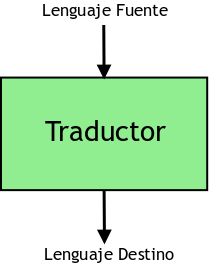
\includegraphics[width=4.5cm,height=6cm]{traductor.png}
		\caption{M\'odulo Traductor}
		\label{gbraun:traductor}
	\end{figure}

        
        A continuaci\'on, especificaremos los lenguajes fuente y
        destino y luego estudiaremos el m\'odulo traductor con m\'as detalle.

	\subsection{El Lenguaje Fuente} \label{cap6:fuente}

        El lenguaje fuente abarca los siguientes
        formalismos definidos en el cap\'itulo \ref{pagcap5}:

        \begin{itemize}

        \item PDDL$_{STRIPS}$. PDDL con el requerimiento
        \texttt{strips}. La expresividad subyacente es equivalente a STRIPS est\'andar.
        
        \item PDDL$_{L}$. PDDL con los requerimientos \texttt{strips} y \texttt{equality}.
        Tambi\'en permite la inclusi\'on de negaci\'on de igualdad en
        precondiciones. El predicado de igualdad y su negaci\'on son soportados por el
        Planificador Continuo y fueron considerados como
        parte del lenguaje fuente aunque no est\'en definidos en STRIPS est\'andar.

        \item PDDL$_{\emph{C}}$. Esta variante PDDL soporta
        \texttt{strips}, \texttt{equality} y
        \texttt{conditional-effects}. Los efectos condicionales
        est\'an restringidos a la definici\'on de un solo antecedente y
        un solo consecuente. Los antecedentes deben ser de la forma \texttt{(= X
        Y)} o \texttt{(not (= X Y))}.

        \item PDDL$_{D}$. PDDL con los requerimientos \texttt{strips},
          \texttt{equality} y \texttt{disjuntive-preconditions}.

        \item PDDL$_{u}$. PDDL con los requerimientos \texttt{strips},
        \texttt{equality} y \texttt{universal-preconditions}. Las precondiciones
        cuantificadas universalmente requieren que el problema defina por un conjunto finito y
        est\'atico de objetos. Todos estos objetos deben ser del mismo tipo.

        \end{itemize}
        
        Cada problema de planificaci\'on de entrada debe estar
        especificado en cualquiera de estos formalismos pertenecientes
        al lenguaje fuente. 

        \subsection{El Lenguaje Destino} \label{cap5:destino}

        Como parte del lenguaje destino, vamos a identificar dos
        representaciones similares. Por un lado, la notaci\'on STRIPS
        gen\'erica que ofrece el traductor y por otro, c\'omo esta
        representaci\'on es adaptada al algoritmo de Planificaci\'on
        Continua.

        El m\'odulo traductor propuesto ofrece una notaci\'on
        gen\'erica que permite personalizar la definici\'on de STRIPS
        seg\'un el algoritmo planificador al que se quiera
        integrar dicho m\'odulo. Esta representaci\'on
        permite reutilizar el traductor en otros
        algoritmos, cuyo lenguaje de representaci\'on sea similar a STRIPS,
        sin la necesidad de modificar los m\'odulos principales de traducci\'on.
        La notaci\'on gen\'erica definida, llamada 
        \emph{Prolog-like}, es la siguiente:


        \begin{itemize}

        \item \emph{Precondiciones, Agregados y Borrados}. Por cada acci\'on en el dominio de
        entrada, el traductor genera los predicados \texttt{preconditions}, \texttt{achieves}
        y \texttt{deletes} respectivamente, con los siguientes
        argumentos: \texttt{action\_name(parameters)} y una lista de
        predicados \texttt{[pre\-di\-ca\-te$_{1}$(pa\-ra\-men\-ters$_{1}$),...,
        predicate$_{N}$(paramenters$_{N}$)]}, donde \texttt{parameters$_{i}$} es
        una lista de variables Prolog separada por comas. 

        \item \emph{Objetos, Meta y Estado Inicial}. El traductor genera un
        predicado \texttt{objects(obj$_{1}$,obj$_{2}$,...,obj$_{N}$)}
        donde \texttt{obj$_{i}$} es un \'atomo
        Prolog. Adem\'as, genera \texttt{goal(fact$_{g}$)} donde \texttt{fact$_{g}$} son
        hechos Prolog de la forma \texttt{fact(parameters$_{g}$)} y 
        \texttt{parameters$_{g}$} es una lista de \'atomos separados
        por comas. Por \'ultimo,
        \texttt{init(fact$_{1}$,fact$_{2}$,..,fact$_{N}$)} es la
        definici\'on del estado inicial
        donde, \texttt{fact$_{i}$} es de la
        forma \texttt{init(parameters$_{i}$)}
        y \texttt{parameters$_{i}$} es una lista de \'atomos separados
        por comas. 
 
        \end{itemize}

        A continuaci\'on, mostramos un ejemplo con la notaci\'on
        gen\'erica definida para el traductor.

        \begin{ejemplo}
        \begin{verbatim}
% Dominio	
preconditions(action_name_1(parameters), 
         [predicate_1(paramenters_1), 
         ...
         predicate_N(paramenters_N)]).   
achieves(action_name_1(parameters),
         [predicate_1(paramenters_1),
         ...
         predicate_N(paramenters_N)]).
deletes(action_name_1(parameters),
         [predicate_1(paramenters_1),
         ...
         predicate_N(paramenters_N)]).

% Problema
(domain(domain_name),
 objects(obj1,obj2,..,objN),
 goal(fact_g),
 init(fact_1,fact_2,..,fact_N)).
        \end{verbatim}
        \end{ejemplo}

        Teniendo en cuenta que uno de los objetivos de nuestra investigaci\'on es
        integrar el m\'odulo al Framework de Planificaci\'on
        Continua, el lenguaje destino del traductor est\'a restringido al lenguaje
        de representaci\'on soportado por el algoritmo de
        planificaci\'on que implementa el framework.
        En este caso, los dominios y problemas de planificaci\'on est\'an
        especificados en STRIPS est\'andar m\'as los predicados
        de igualdad (denotado como \texttt{`=='}) y distinto (denotado
        como \texttt{`\textbackslash =='}).
        Cada acci\'on se compone de un
        predicado \texttt{preconditions}, un nuevo
        predicado \texttt{deletes} por cada predicado en
        la lista de borrados gen\'erica y un predicado \texttt{achieves}
        por cada predicado en la lista gen\'erica de
        agregados.
        Para adaptar los problemas, la traducci\'on es similar. Por cada
        predicado gen\'erico en \texttt{init} se genera un nuevo hecho
        Prolog con la sintaxis \texttt{holds(fact$_{i}$,init)}. 

        Luego, la representaci\'on Ciao Prolog lograda es la siguiente:

        \begin{verbatim}
% action(X,Y,Z)
preconditions(action(X,Y,Z),[pred1(X),pred2(Y),pred3(Z)]):- X == Y,Y \== Z.
achieves(action(X,Y,Z),pred1(X)).
achieves(action(X,Y,Z),pred3(Z)).
deletes(action(X,Y,Z),pred2(Y)).

% Problem
holds(pred1(object1),init).
holds(pred2(object2),init).
holds(pred3,init).
        \end{verbatim}  
        

        A continuaci\'on, detallaremos la
        arquitectura del traductor y analizaremos el comportamiento de
        cada uno de sus m\'odulos.


	\subsection{M\'odulos de la Arquitectura} \label{cap5:modarq}
	
	La arquitectura del traductor est\'a organizada en los
        siguientes m\'odulos:
	
	\begin{itemize}
	
	\item \texttt{pddltostrips}: es el m\'odulo
	``controlador'' y debe incluirse en la especificaci\'on PDDL de entrada
	usando la sentencia Prolog
        \texttt{use\_package(pddltostrips)}. Permite cargar el 
        m\'odulo \texttt{pddltostrips\_tr} y el
	predicado \texttt{parser\_ext} en tiempo de compilaci\'on
        para comenzar la traducci\'on.
	
	
	\item \texttt{pddltostrips\_tr}: este m\'odulo incluye la
        definici\'on del predicado \texttt{parser\_ext}. 
        El pre\-di\-ca\-do recibe un dominio y un problema en PDDL y retorna
        la especificaci\'on STRIPS correspondiente. Interact\'ua con
        los m\'odulos \texttt{tokenizer}, \texttt{parse\_problem}
        y \texttt{parse\_domain}. 
        Este m\'odulo tambi\'en es el que interpreta la
        representaci\'on gen\'erica STRIPS para adaptar el traductor
        al planificador destino.
	
	\item \texttt{pddl\_domain}: usando el paquete \texttt{dcg}, traduce la definici\'on de un
        dominio PDDL, expresado en el lenguaje fuente, a una lista de predicados 
	Prolog en la notaci\'on STRIPS gen\'erica definida en la
        secci\'on anterior. El predicado principal de este m\'odulo es \texttt{parse\_domain}.
	
	\item \texttt{pddl\_problem}: usando el paquete \texttt{dcg}, traduce la definici\'on de un
	problema PDDL, expresado en el lenguaje fuente, a una lista de predicados
	Prolog en la notaci\'on STRIPS gen\'erica definida. El
	predicado principal de este m\'odulo es \texttt{parse\_problem}.
	
	\item \texttt{tokenizer}: este m\'odulo act\'ua como
	analizador l\'exico\footnote{Un analizador l\'exico lee una
	cadena de caracteres de la especificaci\'on en el lenguaje
	fuente y los agrupa en secuencias
	llamadas \emph{lexemas}. Para cada \emph{lexema}, el
	analizador genera un \emph{token} como salida \cite{gbraun:Aho:2007}.} y 
        obtiene los \emph{tokens} de la definici\'on PDDL de entrada.
	
	\end{itemize}
	
	Para utilizar este m\'odulo traductor, la especificaci\'on
	PDDL de entrada debe ser importada desde el planificador destino. 
	Esta especificaci\'on, a su vez, debe importar el
	paquete \texttt{pddltostrips} implementado.
        El am\-bien\-te provisto por Ciao Prolog generar\'a, en compilaci\'on, los
	STRIPS equivalentes y el planificador
	podr\'a hacer uso de ellos para producir un plan.
	La figura \ref{pddl:modules} ilustra la disposici\'on e
        interacci\'on de los m\'odulos mencionados\footnote{Las
        l\'ineas puntuadas entre los m\'odulos representan la
        dependencia entre ellos.}.  
	
	\begin{figure}
	\centering
		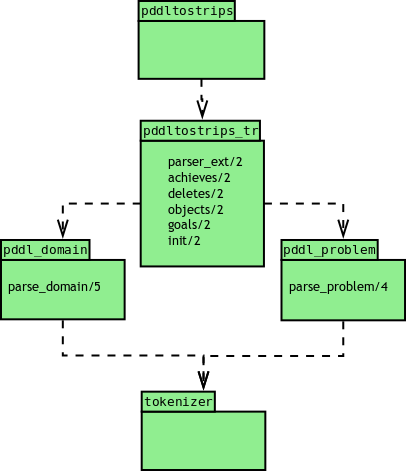
\includegraphics[width=8cm,height=9cm]{UMLParser.png} 
		\caption{Arquitectura Modular del Traductor}
		\label{pddl:modules}
	\end{figure}

        En la secci\'on siguiente analizaremos y
        justificaremos la elecci\'on de Ciao Prolog como el am\-bien\-te
        de programaci\'on ideal para la implementaci\'on del
        traductor PDDL. Tambi\'en, discutiremos brevemente, la noci\'on de expansiones
        sint\'acticas y, en particular, la expansi\'on DCG.

        \section{Ciao Prolog} \label{cap5:Ciao}

	El sistema Ciao \cite{ciao-reference-manual-tr} es un ambiente
        de programaci\'on para el desarrollo de aplicaciones en
        lenguaje Prolog \cite{shapiro:1997:APA:6686} y en varios otros 
        lenguajes que son extensiones y modificaciones de Prolog. 
        Un aspecto importante de Ciao es que, adem\'as de dar soporte 
        para la programaci\'on l\'ogica, prove\'e al programador de un 
        conjunto de caracter\'isticas de diferentes paradigmas y
        estilos de programaci\'on que 
	pueden ser inclu\'idas en cada m\'odulo de un programa. 
        El lenguaje est\'a dise\~{n}ado para ser 
	extendido de una manera simple y modular.
	
	Ciao Prolog presenta el siguiente conjunto de caracter\'isticas:
	
	\begin{itemize}
	
	\item Ofrece un sistema Prolog completo, soportando 
        ISO-Prolog\footnote{International Standard ISO/IEC
        13211-1} \cite{gbraun:estandarprolog}, 
        que permite tanto res\-trin\-gir como expandir el lenguaje
        mediante un sistema modular novedoso.
	
	\item Soporta, a trav\'es de expansiones, programaci\'on
        funcional, restricciones, objetos, registros, 
	persistencia, reglas de control (\emph{breadth-first search}, 
        \emph{iterative deepening}, etc.), concurrencia, 
	ejecuci\'on distribuida y paralela. 
        Tambi\'en incluye librer\'ias para programaci\'on Web (por
        ejemplo, paquetes para manipular lenguaje html, xml, entre otros), sockets e 
	interfaces externas (C, JAVA, Bases de Datos Relacionales, etc.).
	
	\item Ofrece un soporte para programaci\'on a gran escala 
        con un sistema robusto de m\'odulos, compilaci\'on incremental,
        un lenguaje de aserciones para la declaraci\'on de propiedades de programas, 
	inferencia est\'atica y comprobaci\'on est\'atica/din\'amica de tales aserciones.
	
	\item Su compilador genera varias formas de ejecutables 
        \emph{stand-alone}\footnote{Un programa stand-alone
	 es uno que puede ejecutarse como un proceso separado.} e 
         independientes de la arquitectura. 
	 Los m\'odulos de las librer\'ias pueden ser compilados 
         como \emph{bytecode} o como compactos archivos fuentes C y 
         ligados de manera est\'atica, din\'amica o 
	 cargados autom\'aticamente. 
	
	\item Finalmente, es distribuido bajo LGPL 
        GNU\footnote{\emph{Lesser GNU General Public License}.} \cite{gbraun:lgpl}.
	
	\end{itemize}
	
	Ciao es desarrollado por el grupo CLIP de la Universidad
	Polit\'ecnica de Madrid\footnote{CLIP
          Group. \url{http://clip.dia.fi.upm.es/index.html}. Disponible
        en Septiembre de 2012.}.

	
	\subsection{Expansiones Sint\'acticas}
	
	El enfoque orientado a extensibilidad de Ciao posibilita 
	la expansi\'on del lenguaje tanto sint\'actica como
        sem\'anticamente. Estas expansiones pueden ser 
	referenciadas en los m\'odulos, sin interferir con otros,
        gracias a la noci\'on de ``paquetes'' (\emph{packages}).
	
	Una {\bf expansi\'on sint\'actica} \cite{gbraun:exp:sint:2000} 
        toma como entrada una especificaci\'on
        con una determinada sintaxis, posiblemente diferente 
	a la que permite Prolog, y genera una nueva representaci\'on, equivalente 
        a su entrada, que puede ser interpretada en Prolog.
	
	En Ciao, este procesamiento es soportado
        por la directiva \texttt{load\_com\-pi\-la\-tion\_mo\-du\-le/1}. 
	Esta directiva permite separar el c\'odigo que ser\'a usado en tiempo de
        compilaci\'on del c\'odigo que ser\'a usado en tiempo de 
	ejecuci\'on. De esta manera, permite cargar ``en el compilador'', el m\'odulo 
        especificado en su argumento.
	
	Para facilitar la definici\'on de expansiones, Ciao tambi\'en incluye
        cuatro directivas m\'as espec\'ificas. 
	El compilador invoca estos
        predicados en el momento apropiado e 
	instancian su primer argumento con los items a ser
        traducidos. Si el predicado es de aridad 3, 
	el tercer argumento opcional es instanciado con el nombre del 
        m\'odulo donde la traducci\'on se est\'a 
	llevando a cabo (algunas veces necesario durante ciertas
        expansiones). Si la llamada al predicado 
	de expansi\'on es exitosa, el t\'ermino retornado en el
        segundo argumento es usado para reemplazar al original. 
	
	En \cite{gbraun:exp:sint:2000}, Daniel Cabeza y Manuel Hermenegildo, definen las
        siguientes directivas de traducci\'on:
	
	\begin{itemize}
	
	\item \texttt{add\_sentence\_trans/1}: define la traducci\'on
        de t\'erminos, le\'idos por el compilador, 
	en el resto de la entrada actual. 
        Para cada t\'ermino subsecuente, el predicado es nuevamente 
	invocado para obtener un nuevo t\'ermino que ser\'a usado en
        lugar del t\'ermino actual. Un ejemplo 
	de este tipo de traducci\'on es el DCG (\emph{Definite Clause Grammar}).
	
	\item \texttt{add\_term\_trans/1}: define la traducci\'on de
        t\'erminos y subt\'erminos, le\'idos por el compilador, 
	en la entrada actual. Para cada t\'ermino subsecuente, y
        recursivamente, para cada subt\'ermino inclu\'ido, 
	el predicado de traducci\'on es invocado para obtener un nuevo
        t\'ermino en reemplazo del anterior. 
	Esta traducci\'on comienza luego de que todas las traducciones 
        definidas en \texttt{add\_sentence\_trans/1} son ejecutadas.
	
	\item \texttt{add\_goal\_trans/1}: define la traducci\'on de 
        las metas presentes en las cl\'ausulas de la entrada actual. 
	Esta traducci\'on comienza luego de que todas las definidas 
        en \texttt{add\_sentence\_trans/1} y 
	\texttt{add\_term\_trans/1} son ejecutadas.
	
	\item \texttt{add\_clause\_trans/1}: define la traducci\'on de
        las cl\'ausulas de la entrada actual. La traducci\'on 
	comienza antes de \texttt{add\_goal\_trans/1} pero luego de
        las traducciones \texttt{add\_sentence\_trans/1} 
	y \texttt{add\_term\_trans/1}.
	
	\end{itemize}
	
	A continuaci\'on, y en el contexto de estas directivas, podemos analizar el
        m\'odulo \texttt{pddltostrips.pl} de la implementaci\'on propuesta:
	
	\begin{verbatim}
	:- package(pddltostrips). 
	:- load_compilation_module('pddltostrips_tr'). 
	:- add_sentence_trans(parser_ext/2).
	\end{verbatim}


	La primer declaraci\'on indica que \texttt{pddltostrips} es un
        paquete. La directiva 
	\texttt{load\_com\-pi\-la\-tion\_mo\-du\-le} carga, en el compilador, el 
        c\'odigo definido en \texttt{pddltostrips\_tr}. 
	Por \'ultimo, la declaraci\'on \texttt{add\_sen\-ten\-ce\_trans\-(par\-ser\_ext/2)} invoca al predicado 
	\texttt{parser\_ext/2} exportado por \texttt{pddltostrips\_tr}. 
	El predicado realiza la traducci\'on correspondiente en tiempo de compilaci\'on.
	
		
	\subsection{Definite Clause Grammar (DCG)}
	
	La librer\'ia DCG\footnote{Definite Clause Grammars.} es una expansi\'on sint\'actica 
	para las gram\'aticas libres de contexto. Prove\'e a Prolog de
	una notaci\'on conveniente para definir estas gram\'aticas. 
	Las reglas gramaticales son un \emph{syntactic sugar} 
	para cl\'ausulas Prolog ordinarias. Cada regla toma una cadena
	de entrada, analiza alguna subcadena 
	inicial y produce la subcadena restante como salida para un
	posterior an\'alisis. Los argumentos requeridos 
	para las cadenas de entrada y salida no son indicados
	expl\'icitamente en la regla gramatical ya que la sintaxis las define impl\'icitamente.
	
	Una regla DCG en Prolog tiene la siguiente forma:
	
	\begin{verbatim}
	head --> body
	\end{verbatim}
	
	Esto significa que una forma posible para \texttt{head}
        es \texttt{body}. Ambos son secuencias de uno o m\'as \'items 
	ligados por el operador de conjunci\'on est\'andar de Prolog,
        notado como \texttt{`,'}.
	
	La gram\'aticas libres de contexto son extendidas, usando DCG,
	de la siguiente manera:
	
	\begin{enumerate}
	
	\item Un s\'imbolo no terminal puede ser cualquier t\'ermino Prolog.
	
	\item Un s\'imbolo terminal puede ser cualquier t\'ermino
        Prolog. Los s\'imbolos terminales son escritos como 
	listas Prolog y la lista vac\'ia \texttt{[ ]} representa una secuencia vac\'ia de terminales. 
	Si los terminales son caracteres ASCII, los s\'imbolos son escritos como cadenas.
	
	\item Las condiciones extras pueden ser incluidas en el \texttt{body} de la regla gramatical. 
	Las invocaciones se explicitan entre \texttt{\{ \}}.
	
	\item El \texttt{head} de la regla consiste de s\'imbolos no
        terminales. Opcionalmente, puede estar 
	con\-ti\-nua\-do por terminales (en forma de listas).
	
	\item Las alternativas puede definirse en el \texttt{body} 
        utilizando el operador \texttt{`;'}.
	
	\item El s\'imbolo de \emph{cut}, \texttt{`!'}, puede ser 
        incluido en el \texttt{body} de la regla. 
	No es necesario utilizar \texttt{\{ \}}.
	
	\end{enumerate}

        Ilustramos el uso de las DCG con el siguiente ejemplo:
	
        \begin{ejemplo}
        Extraemos el predicado \texttt{pddl2stripsdomain} implementado en el
        m\'odulo \texttt{pddl\_domain} de nuestro traductor.

	\begin{verbatim}
pddl2stripsdomain(Objs,Preconditions, Achieves, Deletes) --> 
  ['(', 'define', '(', 'domain'], name(_Name_Domain),!, [')'], 
  ((requirements_def(Reqs), {_Requirements =..[requirements|Reqs]}) | []),!, 
  ((predicates_def(Dict,Preds), {_Predicates =..[predicates|Preds]}) | []),!, 
  ((constants_def(Consts), {_Constants =..[constants|Consts]}) |[]),!,
  (actions_def(Dict,Objs,Preconditions, Achieves, Deletes) | []),!,
  [')'].
	\end{verbatim}

	Este predicado es invocado desde:
	
	\begin{verbatim}
parse_domain(Input,Objs,Preconditions,Achieves,Deletes)
	\end{verbatim}
	
	Como resultado, retorna las listas
        \texttt{Precondiciones}, \texttt{Agregados} y \texttt{Borrados} 
	co\-rres\-pon\-dien\-tes a la entrada PDDL en el argumento \texttt{Input}.
	\end{ejemplo}
	
        Hasta aqu\'i, hemos presentado los conceptos principales que soportan la
        implementaci\'on de nuestro traductor. Estamos en condiciones
        de analizar paso a paso, a partir de la pr\'oxima secci\'on, la
        implementaci\'on propuesta.

\section{Implementaci\'on del Traductor} \label{cap6:implementacion}

La traducci\'on comienza cuando se invoca, en tiempo de compilaci\'on, 
al predicado \texttt{parser\_ext/2}, cuyo c\'odigo es presentado a
continuaci\'on:

        \begin{verbatim}
parser_ext((Problem,Domain),STRIPS_POP):-
     atom_codes(Problem,CH),
     atom_codes(Domain,CH2),
     tokenizer(CH,TokensProblem),
     tokenizer(CH2,TokensDomain),
     parse_problem(TokensProblem,Objects,Goals,Init),
        
     % Problem customizable predicates to the target planner
     objects_pop(Objects,OBJ_POP),
     goals_pop(Goals,GOALS_POP),
     init_pop(Init,INIT_POP),
     append(OBJ_POP,GOALS_POP,PBL),
     append(INIT_POP,PBL,Problem),

     parse_domain(TokensDomain,OBJ_POP,Preconditions,Achieves,Deletes),

     % Domain customizable predicates to the target planner
     achieves_pop(Achieves,ACHIEVES_POP),
     deletes_pop(Deletes,DELETES_POP),
     append(ACHIEVES_POP,DELETES_POP,D1),
     append(Preconditions,D1,Domain),
     append(Domain,Problem,STRIPS_POP).
        \end{verbatim}


Este predicado recibe como entrada el par \texttt{(Domain,Problem)}
donde \texttt{Domain} y \texttt{Problem} son cadenas de caracteres
escritos como \'atomos Prolog\footnote{Atomos Prolog son cadenas de
caracteres escritos entre comas simples.}.
El predicado Ciao \texttt{atom\_codes} toma estos \'atomos y retorna
la lista de c\'odigos ASCII correspondientes. Ambos, dominio y problema 
PDDL, est\'an en listas separadas de c\'odigos. 

El pr\'oximo paso es generar, a partir de estas listas, secuencias 
significativas del lenguaje PDDL. El predicado
\texttt{tokenizer} implementa esta conducta realizando las siguientes
acciones. Por cada conducta mostramos el fragmento de c\'odigo 
correspondiente.

\begin{itemize}

\item Remueve espacios, saltos de l\'inea y tabulaciones de la lista de
c\'odigos ASCII.

          \begin{verbatim}
%layout spaces,newlines,tabs...
tokenizer([C|RC],Words):- ( C=32 ; C=10 ; C=9 ; C=13 ; C=92 ), !, 
                          tokenizer(RC,Words).
          \end{verbatim}

\item Trata como palabras a los siguientes s\'imbolos:
par\'entesis \texttt{( )}, coma \texttt{`,'}, 
punto \texttt{`.'}, gui\'on medio \texttt{`-'}, dos puntos \texttt{`:'} y al
signo de interrogaci\'on \texttt{`?'}.

         \begin{verbatim}
% Brackets, comma, period or question marks are treated as separed words
tokenizer([C|RC], [Char|Words_1]) :- ( C=40 ; C=41 ; C=44 ; C=45 ;
                                       C=46 ; C=63 ; C=58 ) , 
                                     name(Char, [C]), !,
                                     tokenizer(RC, Words_1).
         \end{verbatim}

\item El resto de los caracteres son retornados como \emph{lexemas}. 
En PDDL estos lexemas son nombres de variables y predicados, palabras
reservadas, constantes y el operador de igualdad \texttt{`='} y
negaci\'on \texttt{not}.

         \begin{verbatim}
% Words
tokenizer([C|RC], [Word|Words_1]):- word([C|RC],Chars,Next), 
                                    name(Word,Chars), 
                                    tokenizer(Next,Words_1).

word([C|RC],[],[C|RC]):- ( C=32 ; C=44 ; C=10 ; C=9 ; C=13 ; C=46 ; 
                           C=63 ; C=40 ; C=41 ; C=58 ; C= -1 ) , !.

word([C|RC],[LC|Chars],Next):- lower_case(C,LC), 
                               word(RC,Chars,Next).
         \end{verbatim} 

\end{itemize}

%tabla de caracteres ASCII para estas listas

En este instante de la traducci\'on tenemos la entrada PDDL reducida 
a listas que ser\'an interpretadas por
las gr\'amaticas definidas en los m\'odulos \texttt{pddl\_problem}
y \texttt{pddl\_domain}.

% PROBLEMAS!

El predicado \texttt{parse\_problem/4} implementado en el
m\'odulo \texttt{pddl\_problem} comienza la traducci\'on del problema
PDDL. Este predicado recibe la lista de \emph{tokens} retornadas por el 
\texttt{tokenizer} y retorna el problema PDDL expresado en la
notaci\'on Prolog gen\'erica definida en la
secci\'on \ref{cap5:destino}. 
La regla principal es analizada a continuaci\'on:

   \begin{verbatim}
pddl2stripsproblem(Objects, Goals, Init) --> 
    ['(', 'define', '(', 'problem'], name(_Name_Problem),!, [')'],
    ['(', ':', 'domain'], name(_Name_Domain), !, [')'], 
    ((objects_def(Objs), {Objects =..[objects|Objs]}) | []),!,  
    ((goals_def(Goal,_,_), {Goals =..[goal|Goal]}) | []),!, 
    ((init_def(Ini), {Init =..[init|Ini]}) | []),!, 
    [')'].
   \end{verbatim}

\texttt{pddl2stripsproblem} retorna los predicados correspondientes a
los objetos, la meta y el estado inicial del problema PDDL. Cada una
de estas secciones es analizada, respectivamente por las siguentes
reglas invocadas: \texttt{objects\_def}, \texttt{goal\_def} e \texttt{init\_def}.

El pr\'oximo paso del traductor es analizar el dominio PDDL, por lo tanto, el
predicado \texttt{parse\_domain/5} es invocado
desde \texttt{parser\_ext} para comenzar la traducci\'on. 
Recibe, como entrada, la lista de \emph{tokens} del dominio PDDL y los
objetos definidos en el problema y 
retorna tres listas: \texttt{Preconditions}, \texttt{Achieves} y \texttt{Deletes}.

La regla principal en este caso es la siguiente:

   \begin{verbatim}
pddl2stripsdomain(Objs,Preconditions, Achieves, Deletes) --> 
    ['(', 'define', '(', 'domain'], name(_Name_Domain),!, [')'], 
    ((requirements_def(Reqs), {_Requirements =..[requirements|Reqs]}) | []),!, 
    ((predicates_def(Dict,Preds), {_Predicates =..[predicates|Preds]}) | []),!, 
    ((constants_def(Consts), {_Constants =..[constants|Consts]}) |[]),!,
    (actions_def(Dict,Objs,Preconditions, Achieves, Deletes) | []),!,
    [')'].
   \end{verbatim}

Cada una de las secciones en la especificaci\'on del dominio PDDL es
analizada por las si\-guien\-tes
reglas: \texttt{requirements\_def}, \texttt{predicates\_def},
\texttt{constants\_def} y \texttt{actions\_def}.

Vamos a estudiar puntualmente la regla \texttt{actions\_def} debido a
que es la que genera las listas STRIPS. El par\'ametro \texttt{Objs}
es la lista de objetos definidos en el problema de planificaci\'on
y \texttt{Dict} es un diccionario de variables, donde cada elemento
del diccionario es un par \texttt{(PDDL
Parameter,Prolog Variable)} para gestionar la correspondencia de
nombres de par\'ametros en predicados. 

El fragmento de c\'odigo para \texttt{actions\_def} es el mostrado a
continuaci\'on.
\ \\

\ \\

        \begin{verbatim}
actions_def(Dict,Objs,Preconditions,Achieves,Deletes) --> 
      ['(',':','action'],name(Name),!, 

      [':', 'parameters'], 
      ['('], list_parameters(Dict,Param),!, [')'],
      {nth(1, Name, Name_Ac),  Ac =..[Name_Ac|Param]},

      [':', 'precondition'], 
      ['('], list_preconditions(Dict,Objs,P),
      {Pre =..[preconditions|[Ac,P]]},!, [')'],
 
      [':', 'effect'], 
      ['('], list_effects(Dict,A, D, P),
      {Ach =..[achieves|[Ac,A]],Del =..[deletes|[Ac,D]]},!, [')'], [')'],

      actions_def(Dict,Objs,PRE2,ACH2,DEL2),!,
      {((instances(P,_),append([Pre],PRE2,Preconditions),
         append([Ach],ACH2,Achieves),append([Del],DEL2,Deletes));
        (generateInstances(Pre,Ach,Del,PRE1,ACH1,DEL1),
         append(PRE1,PRE2,Preconditions),append(ACH1,ACH2,Achieves), 
         append(DEL1,DEL2,Deletes)))}.
        \end{verbatim}


En primer lugar, la regla identifica el nombre de la acci\'on 
mediante el predicado \texttt{name} y pos\-te\-rior\-men\-te,
retorna la lista de par\'ametros declarados para la acci\'on. 
Esta lista es generada desde \texttt{list\_parameters}. 
La regla \texttt{list\_preconditions} inicia la traducci\'on de las
precondiciones de la acci\'on y retorna todos los predicados definidos
para dicha acci\'on. Por \'ultimo, \texttt{list\_effects} retorna los predicados
correspondientes a las listas de agregados y borrados. 
Los efectos negados van a la lista de
borrados y el resto a la de agregados.

Finalmente, el control de la traducci\'on vuelve a \texttt{parser\_ext}. 
En este punto, el traductor permite procesar las estructuras
gen\'ericas definidas para los problemas y los dominios con el
objetivo principal de generar la notaci\'on STRIPS adecuada para el
planificador \emph{target}.
La manipulaci\'on de esta notaci\'on permite el reuso del traductor
sobre diferentes planificadores que utilicen una representaci\'on
similar a STRIPS como lenguaje de representaci\'on.
\ \\

Luego de analizar los fragmentos m\'as importantes de la
implementaci\'on del traductor, en la pr\'oxima secci\'on, vamos a
mostrar c\'omo generar la especificaci\'on PDDL de entrada en Ciao Prolog, c\'omo
invocar el traductor y algunos ejemplos de planificaci\'on utilizando
el algoritmo POP y distintas instancias del ``Mundo de Bloques''. 

   \section{Demostraci\'on del Traductor} \label{cap6:ejemplos}

   Sea el estado inicial para una instancia del ``Mundo de
   Bloques'' tal como indica la figura \ref{demo:estadoInicial}, y la
   meta, como se muestra en la figura \ref{demo:estadoFinal}.

  \begin{figure}[h!]
  \centering
  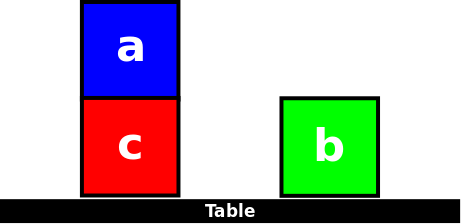
\includegraphics[width=10cm,height=4cm]{bkwInicial.png} 
       \caption{Estado Inicial del ``Mundo de Bloques''}
	\label{demo:estadoInicial}
   \end{figure} 

  \begin{figure}[h!]
  \centering
  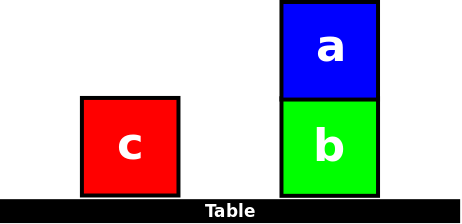
\includegraphics[width=10cm,height=4cm]{bkwFinal.png} 
       \caption{Estado Final del ``Mundo de Bloques''}
	\label{demo:estadoFinal}
  \end{figure}  

  En primer lugar, creamos un archivo llamado \texttt{bkw.pl} y
  definimos el problema y el dominio para esta instancia del ``Mundo de Bloques'' 
  como indica la pr\'oxima figura \ref{demo:pddl}. En esta definici\'on
  incluimos el paquete traductor
  mediante la cl\'ausula Prolog:

  \begin{verbatim}
  :- use_package(pddltostrips.pl).
  \end{verbatim}

  \begin{figure}[h!]
  \centering
  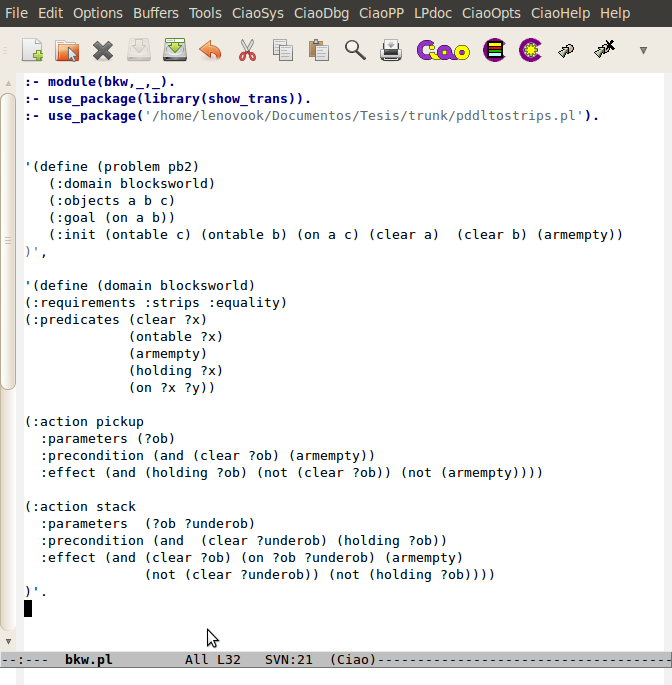
\includegraphics[width=12cm,height=9.5cm]{demoPddlCiao.png} 
       \caption{Especificaci\'on PDDL en Ciao Prolog}
	\label{demo:pddl}
   \end{figure} 

   Luego, desde el planificador (en este caso el POP), referenciamos la especificaci\'on
   PDDL anterior que ser\'a utilizada por el algoritmo
   planificador. Incluimos esta especificaci\'on usando la siguiente
   cl\'ausula, como indica la figura \ref{demo:pop}. 
   
   \begin{verbatim}
   :- use_module(`bkw',[achieves/2,preconditions/2,deletes/2,holds/2]).
   \end{verbatim}   

  \begin{figure}[h!]
  \centering
  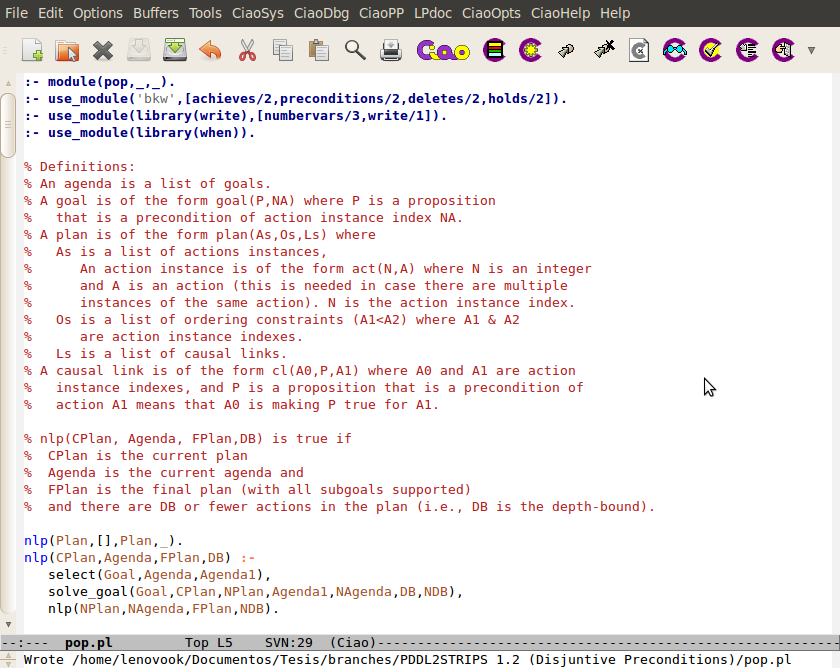
\includegraphics[width=12cm,height=9.5cm]{demoPOP.png} 
       \caption{Planificador POP en Ciao Prolog}
	\label{demo:pop}
   \end{figure}     

   Compilamos y consultamos al planificador con la siguiente
   \emph{query}: \texttt{solve([on(a,b)],P,2), seq(P,S).} para obtener
   un plan.
   Notar que la figura \ref{demo:query} tambi\'en muestra la salida
   del traductor con los STRIPS equivalentes a la especificaci\'on
   PDDL de entrada.

%   \pagebreak

  \begin{figure}[h!]
  \centering
  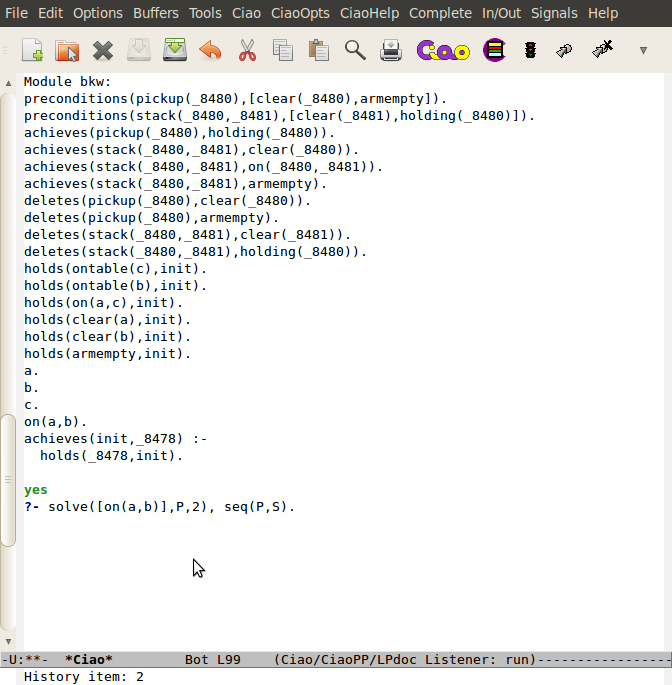
\includegraphics[width=12cm,height=9.5cm]{demoShowtransQuery.png} 
       \caption{Consulta para el planificador POP}
	\label{demo:query}
   \end{figure}

   Por \'ultimo, el planificador retorna el plan deseado que incluye las
   siguientes acciones, como tambi\'en ilustra la figura \ref{demo:plan}:
   \texttt{init, pickup(a), stack(a,b), end}.

  \begin{figure}[h!]
  \centering
  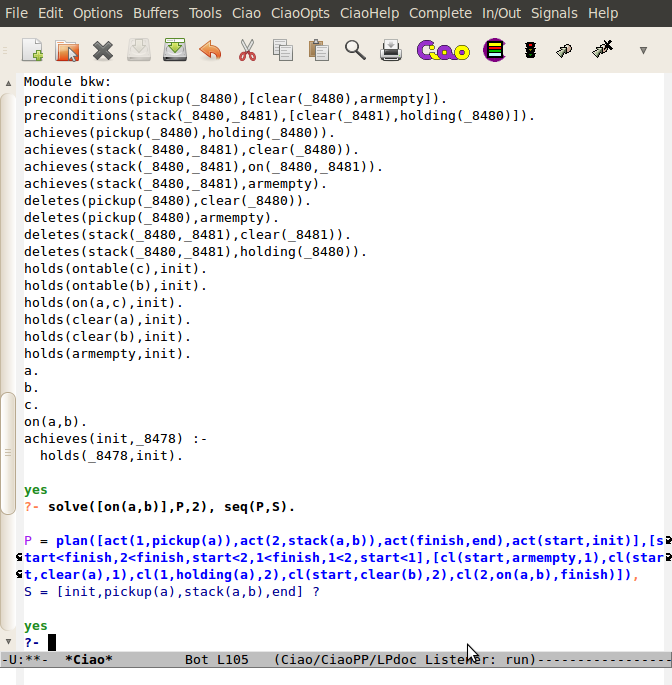
\includegraphics[width=12cm,height=9.5cm]{demoPopPlan.png} 
       \caption{Resultado obtenido de la planificaci\'on}
	\label{demo:plan}
   \end{figure}


   En este cap\'itulo hemos analizado el traductor
   propuesto, definimos su arquitectura y estudiamos el c\'odigo de la
   implementaci\'on. Tambi\'en vimos c\'omo invocar este paquete desde
   Ciao Prolog y c\'omo el traductor es integrado a un planificador
   para poder obtener un plan dada una representaci\'on inicial en
   PDDL.

   En el pr\'oximo cap\'itulo abordamos las conclusiones de esta
   tesis, sus resultados, contribuci\'on y proponemos algunos
   trabajos futuros.

